\begin{figure}[tb]
\centering
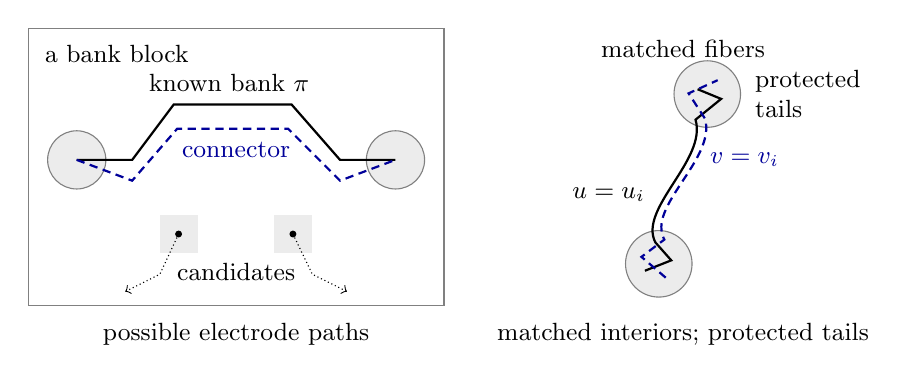
\begin{tikzpicture}[scale=.88,font=\small]
 \begin{scope}
  \draw[gray] (0,0) rectangle (6,4);
  \node[anchor=north west] at (.1,3.9) {a bank block};
  \fill[gray!15] (.7,2.1) circle (.42);
  \fill[gray!15] (5.3,2.1) circle (.42);
  \draw[gray] (.7,2.1) circle (.42) (5.3,2.1) circle (.42);
  \draw[thick] (.7,2.1) -- (1.5,2.1) -- (2.1,2.9)
    -- (3.8,2.9) -- (4.5,2.1) -- (5.3,2.1);
  \node[above] at (2.9,2.95) {known bank $\pi$};
  \draw[blue!60!black,thick,densely dashed]
    (.7,2.1) -- (1.5,1.8) -- (2.15,2.55)
    -- (3.75,2.55) -- (4.5,1.8) -- (5.3,2.1);
  \node[blue!60!black] at (3,2.25) {connector};
  \fill[gray!15] (1.9,.75) rectangle (2.45,1.3);
  \fill[gray!15] (3.55,.75) rectangle (4.1,1.3);
  \fill (2.17,1.03) circle (.05) (3.82,1.03) circle (.05);
  \draw[->,densely dotted] (2.17,1.03) -- (1.9,.45) -- (1.4,.2);
  \draw[->,densely dotted] (3.82,1.03) -- (4.1,.45) -- (4.6,.2);
  \node at (3,.48) {candidates};
  \node[below,align=center] at (3,-.12)
    {possible electrode paths};
 \end{scope}
 \begin{scope}[xshift=7cm]
  \node at (2.45,3.7) {matched fibers};
  \fill[gray!15] (2.1,.6) circle (.48);
  \fill[gray!15] (2.8,3.05) circle (.48);
  \draw[gray] (2.1,.6) circle (.48) (2.8,3.05) circle (.48);
  \draw[thick] (1.9,.5) -- (2.28,.65) -- (2.05,.91)
    .. controls (1.8,1.4) and (2.8,2.1) .. (2.63,2.68)
    -- (3,2.98) -- (2.66,3.12);
  \draw[blue!60!black,thick,densely dashed]
    (2.2,.4) -- (1.85,.7) -- (2.18,.95)
    .. controls (1.92,1.43) and (2.92,2.1) .. (2.77,2.69)
    -- (2.53,3.06) -- (2.95,3.25);
  \node[left] at (2.04,1.6) {$u=u_i$};
  \node[right,blue!60!black] at (2.7,2.1) {$v=v_i$};
  \node[right,align=left] at (3.35,3.05) {protected\\tails};
  \node[below,align=center] at (2.45,-.12)
    {matched interiors; protected tails};
 \end{scope}
\end{tikzpicture}
\caption{The two comparisons in the moving-domain argument, schematically.
Left: a deterministic connector stays near a retained known bank block
while avoiding central candidate neighborhoods; the dots have merely
possible electrode paths, not known open paths or bridges to the bank.
The endpoint balls are charged by the deletion estimate.  Flagged cells,
where an attachment is instead charged by the six-arm estimate, are not
shown.  Right: fibers of the rectangle abscissas $u$ in $U_n$ and $v$ in
$H$ match on compact interior portions; length--area confines their
remaining tails to common small balls.  Neither panel asserts that $H$
and $U_n$ are nested or that their slit boundaries converge uniformly.}
\label{moving:comparison-figure}
\end{figure}
